\documentclass[12pt, a4paper]{article}
\usepackage[utf8]{inputenc}
\usepackage[russian]{babel}
\usepackage{pscyr}

\usepackage{xifthen}
\usepackage{parskip}
\usepackage{hyperref}
\usepackage[top=0.7in, bottom=1in, left=0.6in, right=0.6in]{geometry}
\usepackage{setspace}

\usepackage{amsmath}
\usepackage{MnSymbol}
\usepackage{amsthm}
\usepackage{mathtools}

\usepackage{algorithm}
\usepackage[noend]{algpseudocode}



\linespread{1.2}
\setlength{\parskip}{0pt}

\renewcommand\familydefault{\sfdefault}


% Stuff related to homework specific documents
\newcounter{MyTaskCounter}
\newcounter{MyTaskSectionCounter}
\newcommand{\tasksection}[1]{
	\stepcounter{MyTaskSectionCounter}
	\setcounter{MyTaskCounter}{0}
	\ifthenelse{\equal{#1}{}}{}{
	{\hfill\\[0.2in] \Large \textbf{\theMyTaskSectionCounter \enspace #1} \hfill\\[0.1in]}}
}

\newcommand{\task}[1]{
	\stepcounter{MyTaskCounter}
	\hfill\\[0.1in]
	\ifthenelse{\equal{\theMyTaskSectionCounter}{0}}{
	   \textbf{\large Задача №\theMyTaskCounter}
	}{
	   \textbf{\large Задача №\theMyTaskSectionCounter.\theMyTaskCounter}
	}
	\ifthenelse{\equal{#1}{}}{}{{\normalsize (#1)}}
	\hfill\\[0.05in]
}

% Math and algorithms

\makeatletter
\renewcommand{\ALG@name}{Алгоритм}
\renewcommand{\listalgorithmname}{Список алгроитмов}

\newenvironment{procedure}[1]
  {\renewcommand*{\ALG@name}{Процедура}
  \algorithm\renewcommand{\thealgorithm}{\thechapter.\arabic{algorithm} #1}}
  {\endalgorithm}

\makeatother

\algrenewcommand\algorithmicrequire{\textbf{Вход:}}
\algrenewcommand\algorithmicensure{\textbf{Выход:}}
\algnewcommand\True{\textbf{true}\space}
\algnewcommand\False{\textbf{false}\space}
\algnewcommand\And{\textbf{and}\space}

\newcommand{\xfor}[3]{#1 \textbf{from} #2 \textbf{to} #3}
\newcommand{\xassign}[2]{\State #1 $\leftarrow$ #2}
\newcommand{\xstate}[1]{\State #1}
\newcommand{\xreturn}[1]{\xstate{\textbf{return} #1}}

\DeclarePairedDelimiter\ceil{\lceil}{\rceil}
\DeclarePairedDelimiter\floor{\lfloor}{\rfloor}

\newcommand{\bigO}[1]{\mathcal{O}\left(#1\right)}

\title{Алгоритмы. Домашнее задание №9}
\author{Горбунов Егор Алексеевич}

\begin{document}
\maketitle

\task{Дейкстра и отрицательные веса}
Алгоритм работает следующим образом: изначально в очереди $PQ$ стартовая вершина $s$. Достаём из $PQ$ 
вершину $v$ с минимальной текущей оценкой расстояния $d[v]$. Добавляем вершину $v$ в множество $S$ и релаксируем по всем рёбрам $(v,u)$, инцидентным $v$. Если получилось уменьшить какое-то $d[u]$, то если $u \in PQ$, то делаем $PQ.decrKey(u)$, иначе $PQ.add(u)$. Причём если $u$ принадлежало $S$, то удаляем его из $S$. Выполняем данную процедуру пока не очередь $PQ$ не пуста.\\
\textbf{а)} В силу того, что в графе нет отрицательных циклов от $s$ до любой вершины существует кратчайший путь (пусть
граф связен). Алгоритм завершает работу тогда, когда $PQ$ пуста, а все вершины попали в множество $S$. Таким образом
алгоритм завершается как только все вершины оказались в $S$. Т.к. кратчайший путь от $s$ есть до любой вершины $x$ и
его вес конечен, конечно же, то уменьшать бесконечно $d[x]$ не выйдет и алгоритм рано или поздно закончит свою работу. И найдёт кратчайшие пути в силу того, что это модификация алгоритма Дейкстры :) \xqed

\task{Плохой лабиринт для $BFS$}
Очередь при обходе в ширину на итерации $k$ содержит по крайней мере вершины на расстоянии $k$ от начальной
точки обхода. Попытаемся построить такой лабиринт $n\times n$, что число вершин на некотором расстоянии будет
большим. На помощь призовём фрактал, изображённый на рис~\ref{frac}

\begin{figure}[h!]
	\caption{К задаче 2}
	\centering
	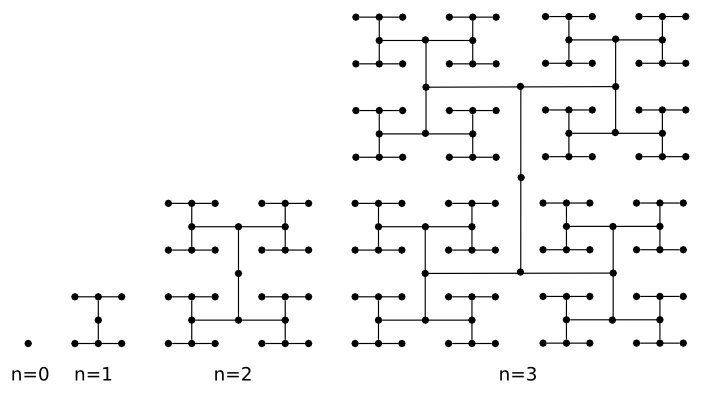
\includegraphics[scale=0.25]{hfrac}
	\label{frac}

\end{figure}

Ясно, что из того, что изображено на рисунке лего получить лабиринт: можем ходить по чёрным линиям, а всё что белое -- это стены. Посмотрим на число вершин, которые находятся на одинаковом
расстоянии от центральной точки этого лабиринта. Пусть сторона лабиринта равна $1$, 
тогда в очереди будет в один момент лишь $1$ элемент. Пусть сторона лабиринта = $3$ ($n=1$ на рисунке). Теперь от центра равноудалены оконечности <<буквы H>> --- их 4 штуки. Аналогично
для стороны лабиринта $=7$, $4*4=16$ вершин попадёт в один
момент в очередь обхода в ширину. Пусть есть лабиринт размера $n$, в котором задана такая фрактальная структура коридоров, причём
размер очереди обхода в ширину достигает $k$ (наибольшее число равноудалённых усиков букв H :) ), тогда можно построить лабиринт со стороной $2n+1$ и получить в нём очередь, при обходе в ширину, размера $4k$! Таким образом увеличение лабиринта вдвое приводит к в 2 раза более быстрому росту размера очереди. Такой лабиринт нам и нужно было найти. \xqed 


\task{Система неравенст} 
$m$ неравенств, $n$ переменных $x_i$, неравенства вида $x_i - x_j \leq \delta_{ij}$. Найти решение за:\\
\textbf{a)} $\bigO{nm}$. Рассмотрим граф $G(V,E)$, $|V| = n + 1$. Вершина $v_i$ соотв. $x_i$. И ещё есть вершина $s$. $\forall v_i:\ (s,v_i) \in E, w(s,v_i) = 0$, где $w(u,v)$ --- вес ребра $(u,v)$.
$(v_j, v_i)\in E, w(v_j,v_i) = \delta_{ij}$, если в системе есть неравенство $x_i-x_j\leq \delta_{ij}$. Запустим алгоритм Беллмана Форда, его результатом будет табличке $d[v_i]$ --- кратчайшее расстояние от $s$ до $v_i$. Заметим, что $d[v_i] \leq d[v_j] + \delta_{ij}$ (неравенство треугольника). А значит, что решение найдено: $x_i = d[v_i]$. Это всё верно, если алгоритм Беллмана-Форда не нашёл цикл отрицательного веса. Если же такой цикл найден: $v_1,v_2,\ldots,v_1$ (нуо), то в неравенствах это запишется так: $x_2 - x_1 \leq \delta_{12},\ldots,x_1-x_k \leq \delta_{1k}$. Просуммировав их у нас всё сократится слева и отрицательное число выйдет справа, т.е. получим неверное утверждение, что отр. число больше или равно 0, а значит система не имеет решений.\\
Алгоритм работает за $\bigO{nm}$\\
\textbf{б)} Если $\delta_{ij}\ geq 0$, решить за $o(nm)$. К тому же графу из п. а) применяем алгоритм Дейкстры: $\bigO{m\log n} = o(nm)$  \xqed
 
\task{Форд-Беллман с порядком на вершинах}
Обозначим множество рёбер из большей вершины в меньшую (причём упоряд. по возрастанию исходящей вершины) за $D$, 
а из меньшей в большую (упоряд. по убыванию исходящей вершины) за $A$.\\
Рассмотрим какой-то кратчайший путь $p$ из $v_1$. В нём всяко не больше $n$ вершин. Если все рёбра на этом пути принадлежат одному множеству: $D$ или $A$, причём в правильно порядке обхода. То описанная в условии задачи процедура правильно прорелаксирует весь путь за 1-ую (проход по $D$) или 2-ую (проход по $A$) половину 1-го этапа. Пускай теперь на $p$ происходит одна единственная смена направления, т.е. до какого-то момента
индексы вершин на пути возрастают, а потом начинают убывать. В таком случае нам нужно выполнить один полный этап, чтобы верно прорелаксировать этот путь. Заметим так же, что первое ребро на пути всегда принадлежит множетству $A$. Легко видеть, что чем больше на пути смен направлений, т.е. мест $v_i,v_j,v_k$, где $i < j$, а $j > k$ или $i > j$, а $j < k$, тем больше нужно этапов для релаксации такого пути. Худший случай:
$v_1,v_n,v_2,v_{n-2},v_3,v_{n-3},v_4,v_{n-4},\ldots,v_{\frac{n}{2}-1},v_{\frac{n}{2}+1}$. Видим, что за каждый этап процедуры мы будем верно релаксировать $2$ последовательных ребра этого пути:
на первом этапе $v_1,v_n,v_2$, причём ребро $v_1,v_n$ будет релаксировано за первую половину процедуры, а $v_n,v_2$ за вторую (проход по $D$). Таким образом видим, что в худшем случае нам нужно $\frac{n}{2}$ этапов. \xqed
\end{document} 